% This is "sig-alternate.tex" V2.0 May 2012
% This file should be compiled with V2.5 of "sig-alternate.cls" May 2012
%
% This example file demonstrates the use of the 'sig-alternate.cls'
% V2.5 LaTeX2e document class file. It is for those submitting
% articles to ACM Conference Proceedings WHO DO NOT WISH TO
% STRICTLY ADHERE TO THE SIGS (PUBS-BOARD-ENDORSED) STYLE.
% The 'sig-alternate.cls' file will produce a similar-looking,
% albeit, 'tighter' paper resulting in, invariably, fewer pages.
%
% ----------------------------------------------------------------------------------------------------------------
% This .tex file (and associated .cls V2.5) produces:
%       1) The Permission Statement
%       2) The Conference (location) Info information
%       3) The Copyright Line with ACM data
%       4) NO page numbers
%
% as against the acm_proc_article-sp.cls file which
% DOES NOT produce 1) thru' 3) above.
%
% Using 'sig-alternate.cls' you have control, however, from within
% the source .tex file, over both the CopyrightYear
% (defaulted to 200X) and the ACM Copyright Data
% (defaulted to X-XXXXX-XX-X/XX/XX).
% e.g.
% \CopyrightYear{2007} will cause 2007 to appear in the copyright line.
% \crdata{0-12345-67-8/90/12} will cause 0-12345-67-8/90/12 to appear in the copyright line.
%
% ---------------------------------------------------------------------------------------------------------------
% This .tex source is an example which *does* use
% the .bib file (from which the .bbl file % is produced).
% REMEMBER HOWEVER: After having produced the .bbl file,
% and prior to final submission, you *NEED* to 'insert'
% your .bbl file into your source .tex file so as to provide
% ONE 'self-contained' source file.
%
% ================= IF YOU HAVE QUESTIONS =======================
% Questions regarding the SIGS styles, SIGS policies and
% procedures, Conferences etc. should be sent to
% Adrienne Griscti (griscti@acm.org)
%
% Technical questions _only_ to
% Gerald Murray (murray@hq.acm.org)
% ===============================================================
%
% For tracking purposes - this is V2.0 - May 2012

\documentclass{sig-alternate}
\usepackage{color}
\usepackage{amsmath}
\usepackage{enumitem}
\usepackage{epstopdf}
\usepackage{url}
\usepackage{graphicx}
\usepackage{hyperref}
\newcommand{\vect}[1]{\boldsymbol{#1}} % Uncomment for BOLD vectors.
\usepackage[tight,footnotesize]{subfigure}
\begin{document}
%
% --- Author Metadata here ---
\conferenceinfo{ACMMultimedia}{'2016 Amsterdam}
%\CopyrightYear{2007} % Allows default copyright year (20XX) to be over-ridden - IF NEED BE.
%\crdata{0-12345-67-8/90/01}  % Allows default copyright data (0-89791-88-6/97/05) to be over-ridden - IF NEED BE.
% --- End of Author Metadata ---

\title{A Perceptual Quality Metric for Videos Distorted by Spatially Correlated Noise}
%
% You need the command \numberofauthors to handle the 'placement
% and alignment' of the authors beneath the title.
%
% For aesthetic reasons, we recommend 'three authors at a time'
% i.e. three 'name/affiliation blocks' be placed beneath the title.
%
% NOTE: You are NOT restricted in how many 'rows' of
% "name/affiliations" may appear. We just ask that you restrict
% the number of 'columns' to three.
%
% Because of the available 'opening page real-estate'
% we ask you to refrain from putting more than six authors
% (two rows with three columns) beneath the article title.
% More than six makes the first-page appear very cluttered indeed.
%
% Use the \alignauthor commands to handle the names
% and affiliations for an 'aesthetic maximum' of six authors.
% Add names, affiliations, addresses for
% the seventh etc. author(s) as the argument for the
% \additionalauthors command.
% These 'additional authors' will be output/set for you
% without further effort on your part as the last section in
% the body of your article BEFORE References or any Appendices.

\numberofauthors{3} %  in this sample file, there are a *total*
% of EIGHT authors. SIX appear on the 'first-page' (for formatting
% reasons) and the remaining two appear in the \additionalauthors section.
%
%\author{
% You can go ahead and credit any number of authors here,
% e.g. one 'row of three' or two rows (consisting of one row of three
% and a second row of one, two or three).
%
% The command \alignauthor (no curly braces needed) should
% precede each author name, affiliation/snail-mail address and
% e-mail address. Additionally, tag each line of
% affiliation/address with \affaddr, and tag the
% e-mail address with \email.
%
% 1st. author
%\alignauthor
%Chao Chen\\
%\affaddr{Google Inc.}\\
%       \affaddr{1600 Amphitheatre Parkway}\\
%       \affaddr{Mountain View, California}\\
%       \email{chaochen@google.com}
%% 2nd. author
%\alignauthor
%Mohammad Izadi\\
%\affaddr{Google Inc.}\\
%       \affaddr{1600 Amphitheatre Parkway}\\
%       \affaddr{Mountain View, California}\\
%       \email{izadi@google.com}
%% 3rd. author
%\alignauthor
%Anil Kokaram\\
%\affaddr{Google Inc.}\\
%       \affaddr{1600 Amphitheatre Parkway}\\
%       \affaddr{Mountain View, California}\\
%       \email{anilkokaram@google.com}
%} 
% There's nothing stopping you putting the seventh, eighth, etc.
% author on the opening page (as the 'third row') but we ask,
% for aesthetic reasons that you place these 'additional authors'
% in the \additional authors block, viz.
% Just remember to make sure that the TOTAL number of authors
% is the number that will appear on the first page PLUS the
% number that will appear in the \additionalauthors section.

\maketitle
\begin{abstract}
Assessing the perceptual quality of videos is critical for monitoring and optimizing video processing pipelines. In this paper, we focus on predicting the perceptual quality of videos distorted by noise. Existing video quality metrics are tuned for ``white", i.e., spatially uncorrelated noise. However, white noise is very rare in real videos. Based on our analysis of the noise correlation patterns in a broad and comprehensive video set, we build a video database that simulates the commonly encountered noise characteristics. Using the database, we develop a perceptual quality prediction algorithm that explicitly incorporates the noise correlations. Experimental results show that the proposed algorithm presents high accuracy in predicting perceptual qualities of noisy videos. 
\end{abstract}

% A category with the (minimum) three required fields
\category{H.5.1}{Information Interfaces and Presentation}
{Multimedia Information Systems Evaluation / methodology}
%A category including the fourth, optional field follows...
\category{C.4}{Performance of Systems}{Design studies}
\category{H.1.2}{Models and Principles}{User/Machine} {Systems/Human factors}

\terms{Performance, Experimentation, Human Factors}

\keywords{Subjective Video Quality Assessment, Noise, Power Spectrum Density}
\section{Introduction}
During video acquisition, compression and communication, various types of distortion may be introduced. Among them, noise is typically introduced in the acquisition process, and it may propagate throughout the video processing and communication pipeline. Accurately predicting the impact of noise on perceptual quality helps in optimizing the overall efficiency of video services. For example, using the estimated noise level, we may be able to predict the likelihood of severe blocking in a subsequent transcoding operation\cite{AlMer1999}. We can then select a suitable pre-processor to reduce the knock-on effects both on bitrate and quality.

The best way of assessing video quality is to collect human scores by conducting subjective tests. However, human studies are labor intensive and not applicable to real-time applications. It is, therefore, appealing to devise an algorithm that can accurately predict perceptual quality. Perceptual image and video quality prediction have been extensively studied, and several high-performance metrics have been invented. For image quality prediction, SSIM\cite{SSIM} achieves very high correlation with perception and has been widely used due to its low complexity. For video quality prediction, MOVIE\cite{MOVIE} and STMAD\cite{STMAD} report the best accuracy. 

A common drawback of these high-performance metrics is that they need a pristine example of the video clip under test. In practice, for instance in quality assessment of YouTube uploads, such a reference is unavailable. This limitation motivated research on no-reference image/video quality metrics. One approach to this problem is to measure the ``unnaturalness" of a picture or a video. It has been found that certain statistics of a pristine image/video follow certain models\cite{SriLeeSimZhu2003}\cite{ZorWei2009}. Quality can then be evaluated by measuring the deviation of these statistics from the models. The image quality metrics proposed by \cite{NIQE}, \cite{DIIVINE}, \cite{HNR} and video quality metrics proposed by \cite{BLIINDS} and \cite{ZhuLiAsaSau2015} follow this methodology. Another method of no-reference quality prediction is based on the free-energy principle in brain science\cite{Fri2010}. In this theory, when a visual signal is perceived, the human brain tries to infer the signal using an internal generative model. The free energy of this inference process, i.e., the discrepancy between the visual signal and the inference of the internal generative model thus can be used to quantify the level of distortion. The algorithms proposed in \cite{LiuZhaZhaSunGuYan2014} and \cite{ZhaWuYanLinZha2012} follow this method to predict image quality.

Besides the aforementioned general-purpose quality metrics, several algorithms are specifically designed for noise \cite{LimPar2014,ZhaKauWanYan2013,ZhaWu2011}. These algorithms, along with the general-purpose algorithms are designed or tuned for predicting the videos distorted by white noise. However, the noise on neighboring pixels is typically correlated. As demonstrated in \cite{SeyKeiKnoSte2013}, the demosaicing operation in video acquisition is performed over neighboring pixels and thus introduces correlation. We verified this in the videos uploaded to YouTube and found that the noise all presents some degree of correlations (see section \ref{sec:noise_analysis} for more details).

In this paper, we propose a no-reference video quality metric for realistic noise. To this end, we first analyzed the noise correlation patterns on a vast and comprehensive video set. Using the typical noise correlation patterns we found in the video set, we construct a video database that simulates the commonly encountered noise. A series of subjective tests are then performed to evaluate the perceptual quality of the noisy videos in the database. Then, we develop a perceptual quality metric that explicitly incorporates noise correlation patterns in quality prediction. Experimental results show that the proposed algorithm can accurately predict the perceptual quality of noisy videos. 

The rest of the paper is organized as follows: section~\ref{sec:noise_quailty_database} describes the construction of our quality database for practical noisy videos. Section~\ref{sec:quality_metric} details the proposed quality metric. Section ~\ref{sec:experiment} shows the performance of the proposed metric. The paper is concluded in section~\ref{sec:conclusion}

\section{Constructing the Database}
\label{sec:noise_quailty_database}
Since the number of sample videos in a subjective test session is limited, they should be carefully selected to represent noise patterns observed in practice. We analyzed the noise structure of a large set of consumer generated videos. Based on the distribution of the noise structures, we created a series of test videos that are representative. The perceptual quality of the videos is then assessed in a series of subjective tests for the development of our quality prediction algorithm.
\subsection{Realistic Noise Analysis}
\label{sec:noise_analysis}
Every type of video capture pipeline may present different noise statistics. Hence, there exist many different noise structures in practical videos. YouTube is a video-sharing platform with an enormous amount of consumer-generated video contents. We collect 46,000 videos uploaded to YouTube to analyze their noise patterns. These videos are selected such that
\begin{itemize}[leftmargin=*]
\setlength\itemsep{-0.2em}
\item They represent varying contents e.g. sports, movies, nature, music video, etc. 
\item They are captured with over 200 different types of cameras or device models.
\item They represent varying resolutions including 360p, 720p, 1080p, 2K and 4K.
\item Their length is longer than 30 seconds to focus on contents that have a chance of being watched. 
\end{itemize}

We analyze the noise patterns of the video collection with a 2D auto-regressive (AR) model. This model has been widely used to analyze noise structure and synthesize film grain \cite{DeStefano2006,ColRobWhi2004}. Denoting by $\mathsf{N}(x,y)$ the synthesised noise at position $(x,y)$, the AR model is:
\begin{equation}
\label{eq:ar_noise_model}
\mathsf{N}(x,y) = \sum\limits_{(i,j) \in \mathcal{S}_\Delta} {w_{i,j}.\mathsf{N}(x+i,y+j)}+\mathsf{G}^{\sigma}(x,y),
\end{equation}
where $\mathsf{G}^{\sigma}(x,y) \sim {\cal N}(0,\sigma^2)$ is
a Guassian random variable with zero mean and variance $\sigma^2$. The set $\mathcal{S}_\Delta$ is the square neighborhood of $(0,0)$ with size $(2\Delta + 1)\times(2\Delta + 1)$. The noise at a pixel $(x,y)$ is modeled as the sum of a white noise sample and a weighted sum of the noise in its neighborhood. The weight assigned to the pixel at $(x+i,y+j)$ is the model parameter $w_{i,j}$. Note that this is a prediction equation and so $w_{i,j} = 0$ for the pixels succeeding to the center pixel in raster-scan order. In the following we denote by $\vect{w}$ the vector of weight parameters, i.e., $\vect{w} = \left(w_{i,j}: \forall (i,j)\in\mathcal{S}_\Delta\right)^\mathsf{T}$. The parameter $\sigma^2$ characterizes the power of noise. For a fixed $\vect{w}$, larger $\sigma^2$ leads to larger noise power.

To analyze the structure of the noise in a video sequence we employ aspects of the noise estimation method proposed in \cite{KokKelDenCra2016}. That method estimates the Power Spectral Density of the noise in texture-less areas of video frames. This idea has been used in well-known post-production toolkits e.g. \href{http://www.thefoundry.co.uk}{NUKE} and Neat Video. The rationale of this method is that the noise is easier to separate in flat regions of a frame. The method first searches for flat patches from all the frames in a video and then applies hyper-planes to approximate the true values of the patches. The approximation error on the patch is considered as the noise. We applied this method on our video collections and fit the AR model to the separated noise to obtain minimum mean square error estimations for the model parameters $\vect{w}$ and $\sigma$. From this analysis, we have the following observations:
\begin{enumerate}[leftmargin=*]
\item An AR model with $\Delta=4$ is sufficient to model the noise in all the 46000 clips ($\Delta>4$ did not improve the fitting error significantly compared to $\Delta=4$). This implies that the noise at two pixels separated by a distance of $>4$ is uncorrelated in a typical video. In the following analysis, we use $\Delta=4$.
\item The histogram of $||\vect{w}||_2$ estimated on the video collection is shown in Figure \ref{fig:w2_histogram}. According to \eqref{eq:ar_noise_model}, $\vect{w}$ reflects the correlation among neighboring pixels. As $||\vect{w}||_2^2$ decreases to zero, the noise $\mathsf{N}(x,y)$ converges to white noise $\mathsf{G}(x,y)$. It is shown in the figure that a large fraction of videos in our collection has non-zero $||\vect{w}||_2^2$. This observation suggests that the noise in real videos is not white in general.
\item We note that the estimation of the model parameter $\vect{\hat w}$ and $\hat\sigma$ may be inaccurate. For videos with textures, the noise separation method may confuse the texture with noise and overestimate the correlation. Therefore, we cannot directly use the noise pattern obtained from the video collection to synthesize the noise for our subjective test.  
\end{enumerate}

\begin{figure}[!hb]
	\centering
	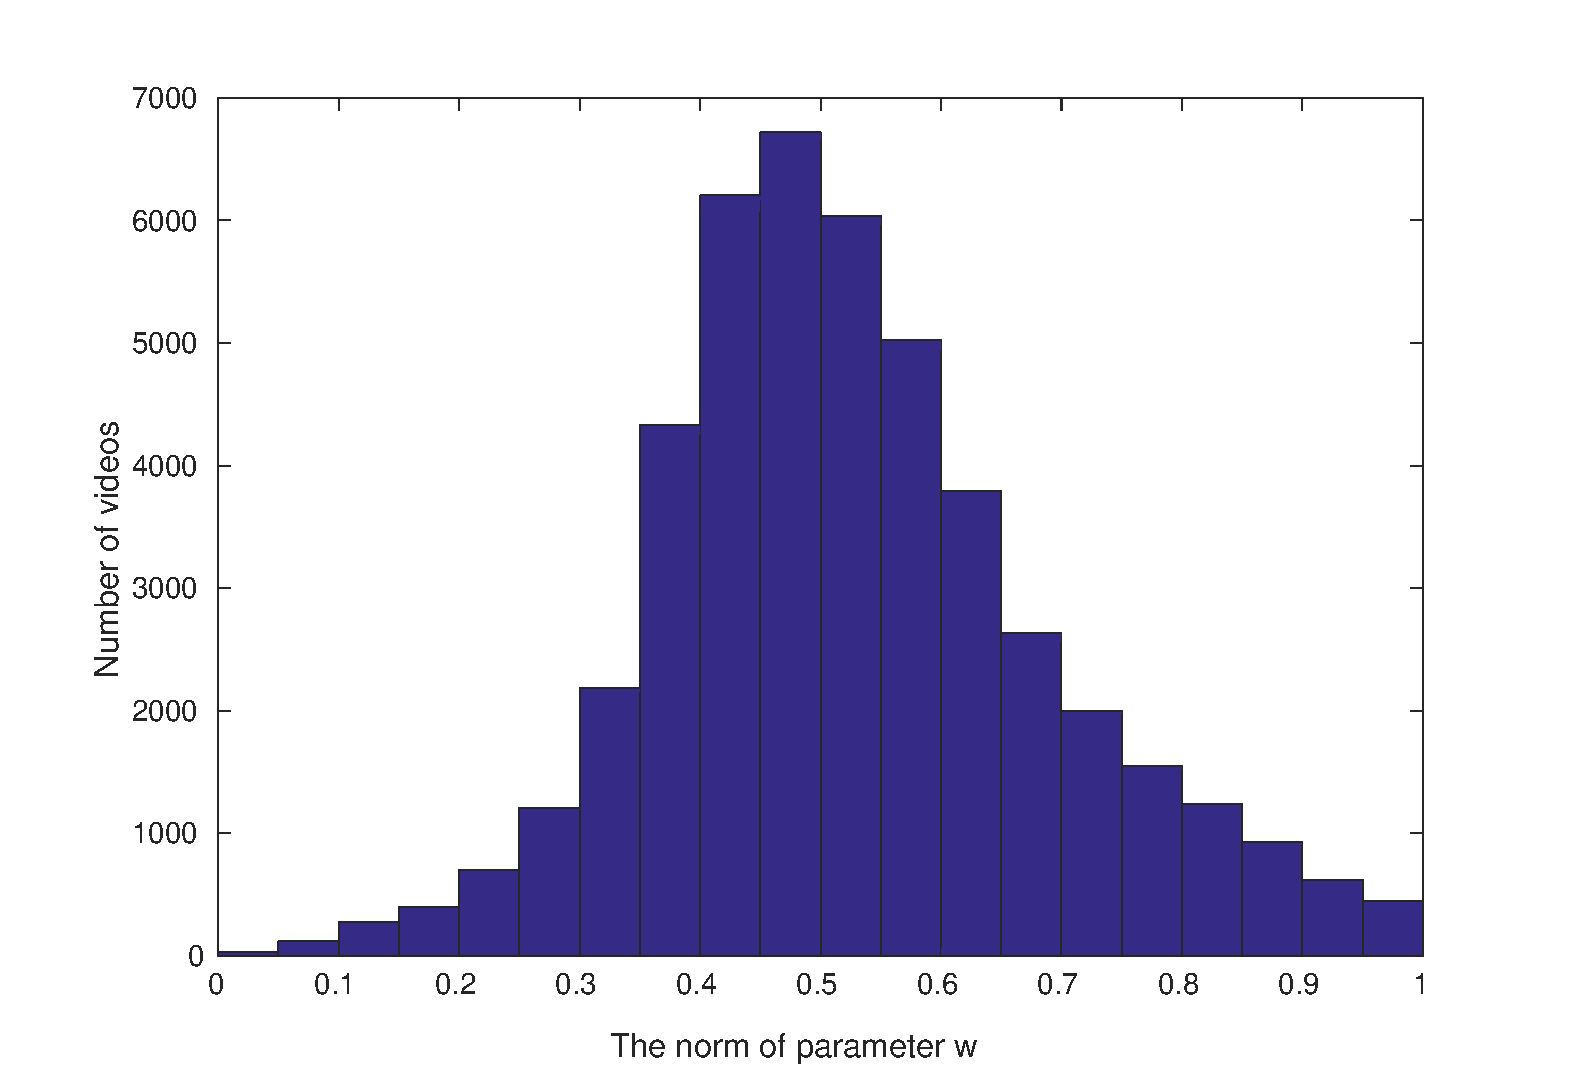
\includegraphics[width=\columnwidth]{img/w2_hist_20.eps}
	\caption{\label{fig:w2_histogram} The histogram of $||\vect{\hat w}||_2^2$ estimated on a video collection of 46000 videos.}
\end{figure}

For $\Delta=4$, the number of non-zero weights $w_{i,j}$ of our AR model is $((2\Delta+1)^2-1)/2=40$. To find out the most typical noise pattern, we may perform a Principal Component Analysis (PCA) on all the $\vect{\hat w}$ in the 40-dimensional space and use the eigenvectors as typical noise patterns for noise synthesis. However, as discussed above, the estimated $\vect{\hat w}$ may contain outliers, and PCA is not robust for the analysis of data with outliers \cite{Bishop2006}. 

To rule out poorly estimated vectors $\vect{w}$, we applied K-means clustering \cite{kmeans} to cluster the estimated vectors into  $\mathrm{K}$ groups. We vary the number of groups $\mathrm{K}$ from $3$ to $15$ and, for a given $\mathrm{K}$, calculate the mean vector of each group as $\left\{\vect{\bar w}^\mathrm{K}_\ell: 1\leq\ell\leq\mathrm{K}\right\}$. Thus we obtain the least correlated and most correlated noise parameter as
\begin{equation}
\vect{\bar w}^\mathrm{K}_\mathrm{min} = \operatorname*{arg\,min}_{\vect{\bar{w}}^\mathrm{K}_\ell}||\vect{\bar w}^\mathrm{K}_\ell||_2,
\end{equation}
and 
\begin{equation}
\vect{\bar w}^\mathrm{K}_\mathrm{max} = \operatorname*{arg\,max}_{\vect{\bar w}^\mathrm{K}_\ell}||\vect{\bar w}^\mathrm{K}_\ell||_2,
\end{equation}

We observed that both $\vect{\bar w}^\mathrm{K}_\mathrm{min}$ and $\vect{\bar w}^\mathrm{K}_\mathrm{min}$ is not changing further as we increase $\mathrm{K}$ over $10$. Therefore, we fix $\mathrm{K}=10$ and define a linear interpolation function between $\vect{\bar w}^\mathrm{10}_\mathrm{min}$ and $\vect{\bar w}^\mathrm{10}_\mathrm{max}$ as:
\begin{equation}
\label{eq:linear_pattern}
\mathbf{w}(\alpha) = \vect{\bar w}^\mathrm{10}_\mathrm{min} + \alpha\left(\vect{\bar w}^\mathrm{10}_\mathrm{max}-\vect{\bar w}^\mathrm{10}_\mathrm{min}\right).
\end{equation}
For any $\alpha\in(0,1)$, $\mathbf{w}(\alpha)$ gives a noise pattern with intermediate correlation level between $\vect{\bar w}^\mathrm{10}_\mathrm{min}$ and $\vect{\bar w}^\mathrm{10}_\mathrm{max}$. To verify that this interpolation yields points close to the 10 clusters, we computed the mean distance of $\vect{\bar w}^\mathrm{10}_\ell$s (excluding $\vect{\bar w}^\mathrm{10}_\mathrm{min}$ and $\vect{\bar w}^\mathrm{10}_\mathrm{max}$) from the interpolating line, normalized by the length between $\vect{\bar w}^\mathrm{10}_\mathrm{min}$ and $\vect{\bar w}^\mathrm{10}_\mathrm{max}$. The normalized mean distance of 0.11 indicates that the line is fairly close to the cluster centers. We also project all $\vect{\bar w}^\mathrm{10}_\ell$s on the interpolating line and compute the distance between every two neighboring projected points on that line. The standard deviation of the gaps is around 0.08 of the length, which implies $\vect{\bar w}^\mathrm{10}_\ell$s are reasonably scattered along the line. In sum, the noise patterns given by \eqref{eq:linear_pattern} provides a reasonable approximation for realistic noise patterns.

\subsection{Test Clip Generation}
The visual quality of a clip depends both on the level of noise and the spatio-temporal characteristics of the video. Therefore, we need to include videos that represent a broad spectrum of spatial and temporal complexities in our test. A simple way to evaluate the spatial/temporal complexity is to measure the average size of their I frames and P frames. However, videos with large I frames tend to have large P frames because high spatial complexity also gives rise to more prediction residuals in motion compensation. To decouple the correlation between I frame size and P frame size, we normalize the size of P frame by the I frame size and use $\frac{\mathrm{P\ frame\ size}}{\mathrm{I\ frame\ size}}$ as the indicator for the temporal complexity. We selected 3226 video clips with 4K resolutions from YouTube such that their encoding bit rates are all higher than 100 Mbps, hence ensuring that they contain minimal noise at source. We then encoded them using the H.264 encoder with FFmpeg. To make the frame size comparable across different videos, we apply a constant quantization parameter of 28 to all videos. The distribution of spatial-temporal features is shown in Fig.~\ref{fig:distribution}. It is seen that the values of the I frame sizes and the normalized P frame sizes are scattered widely and loosely coupled.
\begin{figure}[!hb]
	\centering
	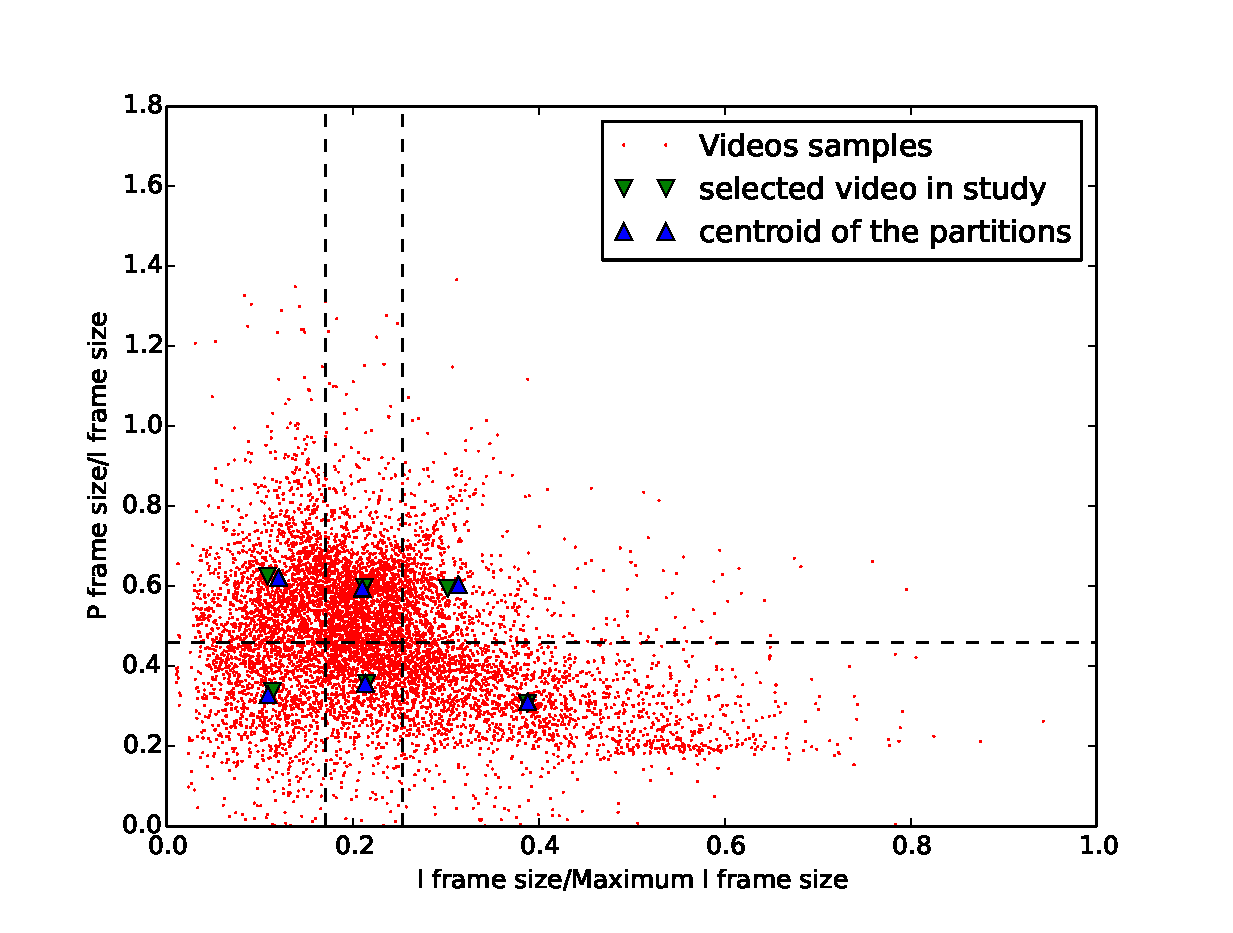
\includegraphics[width=\columnwidth]{img/distribution.eps}
	\caption{\label{fig:distribution} The joint distribution of I frame size and $\frac{\mathrm{P\ frame\ size}}{\mathrm{I\ frame\ size}}$ of 3226 high quality 4K videos uploaded to YouTube.}
\end{figure}

We partition the space of I frame size and normalized P frame size using the percentile of their marginal distributions, respectively. In particular, we calculated the 33\% and 66\% percentile of the marginal distribution of I frame size and the 50\% percentile of the normalized P frame size, respectively. Then we partition the space of spatial-temporal complexity using these percentiles into six regions as shown in Figure \ref{fig:distribution}. In each region, we selected 20 videos that are closest to the centroid of the region (shown by the $\bigtriangledown$ markers in Figure \ref{fig:distribution}). We manually reviewed each of these 20 clips and selected one video that was free from noise and other artifacts such as out-of-focus and over-exposure (shown by $\triangle$ markers in Figure \ref{fig:distribution}). The chosen videos are shown to be close to the centroid of the respective regions and thus are representative of a wide range of spatial-temporal complexity. From each video, we extract a 10-second clip and resize the video from 4K to 1080p resolution. The sample frames of the six clips are shown in Fig.~\ref{fig:sampleframe}.

\begin{figure}[!h]
\centering
\subfigure[beach]{
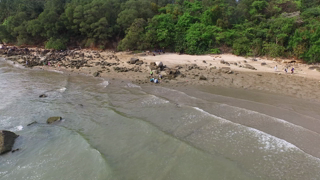
\includegraphics[scale=0.3]{./img/beach.png}

}
\subfigure[goose]{
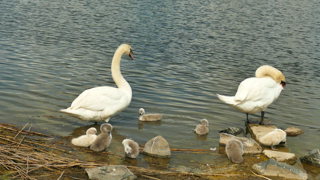
\includegraphics[scale=0.3]{./img/goose.png}

}
\subfigure[singer]{
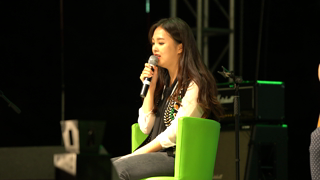
\includegraphics[scale=0.3]{./img/singer.png}

}
\subfigure[snow]{
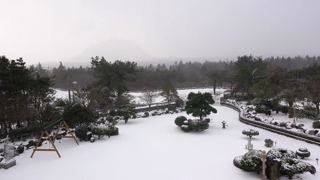
\includegraphics[scale=0.3]{./img/snow.png}

}
\subfigure[sony]{
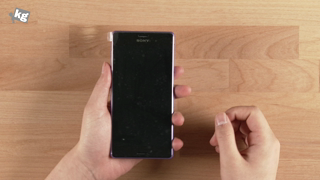
\includegraphics[scale=0.3]{./img/sony.png}

}
\subfigure[talkingman]{
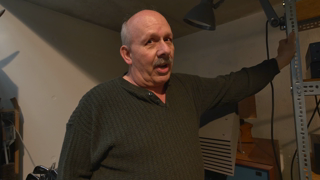
\includegraphics[scale=0.3]{./img/talkingman.png}
}
\caption[Optional caption for list of figures]{
Sample frames of the video clips involved in the subjective test.
}
\label{fig:sampleframe}
\end{figure}

We then employ the AR model \eqref{eq:ar_noise_model} to synthesize noise. We considered 3 models, $\mathbf{w}(0)$, $\mathbf{w}(0.5)$ and $\mathbf{w}(1)$, where $\mathbf{w}(\cdot)$ is defined in \eqref{eq:linear_pattern}. The noise synthesized using the three parameters thus present low, medium, and high noise correlations, respectively. For each noise pattern, we select 4 different $\sigma$ to create 4 test clips with different noise strength. We manually checked the 4 clips to make sure their perceptual quality is visually distinguishable and covers a wide range. In total, we created $3\times4=12$ distorted versions for each video. Because the duration of a test session is limited to be less than 30 minutes, 9 randomly sampled examples from each set of 12 clips were used for our subjective test. Thus, we used $6\times9=54$ clips in total.
\subsection{Subjective Experiment}
\label{sec:subjective_study}
We conducted a Double Stimulus Continuous Quality Scale (DSCQS) subjective test following the ITU guidelines\cite{ITU}. We use a 55 inch Samsung TV for our test, and the participants sit 2.0m away from the screen. 
The screen of the 3840x2160 display was equally split into two parts. The original video and the noisy video were synchronously played in the two parts such that the subjects could view and compare the two clips easily. There were 28 subjects involved in the test. After each pair of clips had been played, the subject was asked to grade the test video using the original video as a reference.

Fig.~\ref{fig:mos} shows the Mean Opinion Scores (MOS) obtained from the subjective test versus the power of the synthesized noise in each test video. The plot demonstrates that, as the power of noise increases, the perceptual quality tend to decrease. However, the noise power itself cannot provide a good prediction for MOS. The rank-order correlation between noise power and MOS is only 0.755.  
\begin{figure}[!hb]
	\centering
	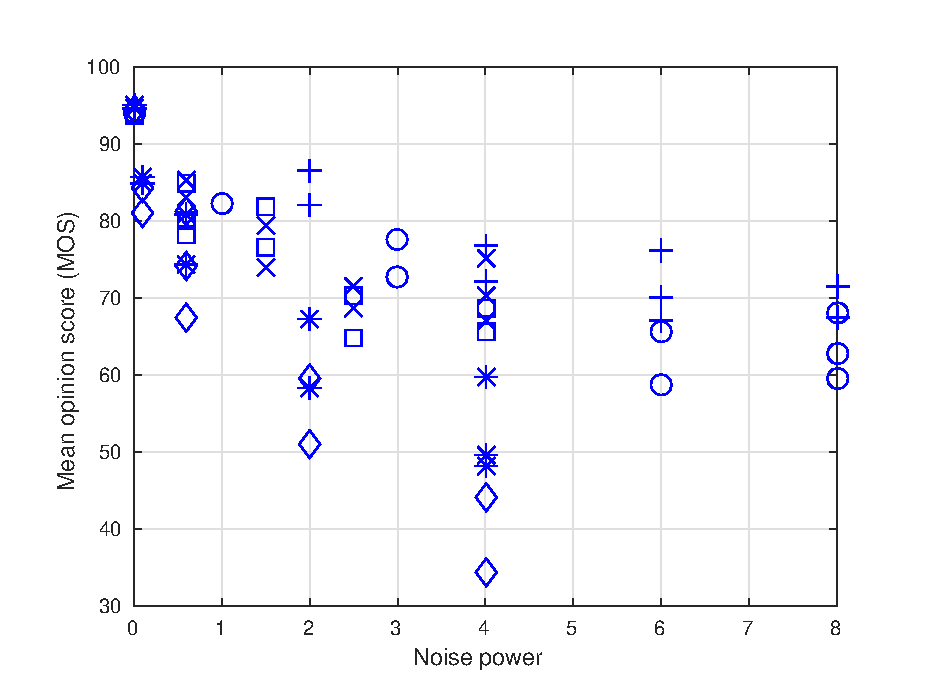
\includegraphics[width=\columnwidth]{img/MOS.eps}
	\caption{\label{fig:mos} The Mean Opinion Scores of the test videos.}
\end{figure}

We also analyzed the relation between noise correlation and MOS. The average MOS for the test clips distorted by noise of low, medium, and high correlation are 76.11, 70.88, and 68.7, respectively. It seems videos with highly correlated noise tend to have worse quality. 

In sum, the perceptual quality of noisy video depends not only on noise power but also on video contents and the structure of noise. In the next section, we present a no-reference quality metric that can accurately predict perceptual qualities by taking into account the noise pattern and video characteristics.

\section{Perceptual Quality Metric}
\label{sec:quality_metric}
The flow chart of the proposed no-reference perceptual quality prediction algorithm is shown in Fig.~\ref{fig:flow_chart}. The noise is first extracted from an input video. Then, the Power Spectral Densities (PSD) of the noise and the input video are estimated in the frequency domain, respectively. For a given frequency channel, the ratio between the PSD of the noise and that of the input video (biased by a regularizing constant $\alpha$) are considered as the noise features of that frequency channel. These features are further adjusted according to the brightness of the video to incorporate contrast sensitivity. A visual importance pooling method is applied to the adjusted features to estimate the visibility of noise in each frequency. The final quality metric is then calculated by summing the estimated visibility over the frequencies that show high correlation with subjective quality. Details follow. 
\begin{figure*}
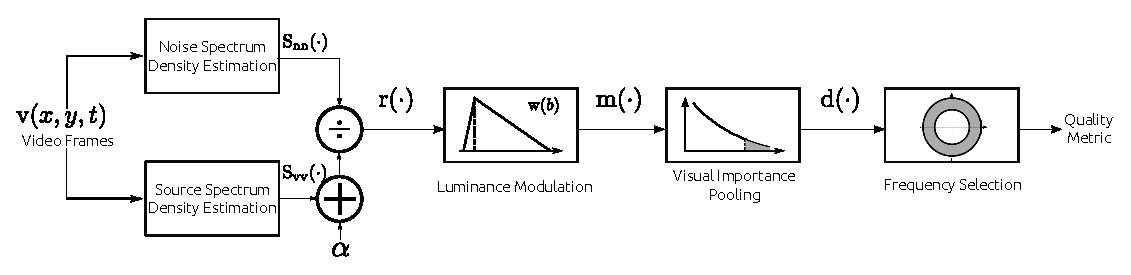
\includegraphics[width=\textwidth]{img/flow_chart.eps}
\caption{\label{fig:flow_chart}The flow chart of the proposed noisy video quality metric.}
\end{figure*}

\subsection{Noise Feature Extraction}
We denote by $\{\mathrm{v}(x,y,t): 0\leq x< W, 0\leq y < H, t\in\mathbb{N}^+\}$ a noisy video signal with resolution $W\times H$. To analyze the local characteristics of the video, we partition the video frames into $B\times B$ non-overlapping blocks and denote by $\{\mathrm{v}^{p,q}(x,y,t)=\mathrm{v}(Bp+x,Bq+y,t): 0\leq x,y < B\}$ be the $(p,q)$'th block of a frame. 

We model $\mathrm{v}^{p,q}(x,y,t)$ as the sum of a noise-free video block $\mathrm{u}^{p,q}(x,y,t)$ and a noise signal $\mathrm{n}(x,y,t)$, i.e.,
\begin{equation}
\mathrm{v}^{p,q}(x,y,t) = \mathrm{u}^{p,q}(x,y,t) + \mathrm{n}^{p,q}(x,y,t),
\end{equation}
where $\mathrm{n}^{p,q}(x,y,t)$ is a realization of a zero-mean random variable $\mathsf{N}(x,y)$. 

As shown in \cite{Bov2013,Dau1985,OlsFie2005}, the visual cortex of human brain decomposes the received visual signal into different orientations and frequencies. In fact, as shown in \cite{Gir1989,MOVIE}, an over-complete wavelet transform can be used to imitate such behavior and extract spatial-temporal features for visual quality prediction. In this paper, we approximate the frequency decomposition in visual cortex using the 3D Discrete Fourier Transform (3D-DFT) and propose to use the ratio of power spectrum density (PSD) of $\mathrm{n}^{p,q}(\cdot)$ and $\mathrm{v}^{p,q}(\cdot)$ as the noise feature. 

For a discrete video signal $\{\mathrm{f}(x,y,t):0\leq x,y<B, 0\leq t<T\}$, its 3D-DFT is given by
\begin{equation*}
\label{eq:dft}
\mathrm{\hat f}(\ell_x,\ell_y,\ell_t)=\sum_{t=0}^{T-1}\omega_T^{\ell_t t}\left(\sum_{y=0}^{B-1}\omega_B^{\ell_y y}\left(\sum_{x=0}^{B-1}\mathrm{f}(x,y,t)\omega_B^{\ell_x x}\right)\right).
\end{equation*}
Here, $\omega_B=\exp(-2\pi\mathrm{i}/B)$ and $\omega_T=\exp(-2\pi\mathrm{i}/T)$ are spatial and temporal discrete Fourier basis, respectively. The PSD of $\mathrm{f}(x,y,t)$ \footnote{Strictly speaking, $\mathrm{S_{ff}}$ should be called periodgram.} is defined by
\begin{equation}
\label{eq:psd}
\mathrm{S_{ff}}(\ell_x,\ell_y,\ell_t) = |\mathrm{\hat f}(\ell_x,\ell_y,\ell_t)|^2.
\end{equation}
PSD captures the signal energy corresponding to spatial frequency $(2\pi\ell_x/B,2\pi\ell_y/B)$ and temporal frequency $2\pi\ell_t/T$. We define the following distortion feature:
\begin{equation}
\label{eq:feature}
\mathrm{r}(\ell_x,\ell_y,\ell_t)=\frac{\mathrm{S_{nn}}(\ell_x,\ell_y,\ell_t)}{\mathrm{S_{vv}}(\ell_x,\ell_y,\ell_t) + \alpha},
\end{equation}
where $\mathrm{S_{nn}}$ and $\mathrm{S_{vv}}$ are the PSDs for noise $\mathrm{n}(x,y,t)$ and video signal $\mathrm{v}(x,y,t)$, respectively. The constant $\alpha$ is a employed to stabilize potential numerical errors. The feature $\mathrm{r}(\ell_x,\ell_y,\ell_t)$ therefore gives the relative noise strength at a given spatial-temporal frequency.  

Another motivation for using $\mathrm{r}(\cdot)$ as the distortion feature is that it captures the correlation pattern of noise. In fact, it can be shown that the PSD of a signal equals to the Fourier transform of its auto-correlation function. The correlation pattern of noise is captured by $\mathrm{S_{nn}}$ and thus by $\mathrm{r}(\cdot)$. 

In our implementation, we fix the blocksize to be $B=32$ and the temporal length to be $T=3$. For each block in a video frame, we concatenate the block with the two co-located blocks in the adjacent frames to form a 3-D array, i.e., $\{\mathrm{v}^{p,q}(x,y,t-1),\mathrm{v}^{p,q}(x,y,t),\mathrm{v}^{p,q}(x,y,t+1): 0\leq x,y<32\}$. Then the 3D-FFT is applied to the array to obtain $\{\mathrm{S}_\mathrm{vv}^{p,q,t}(\ell_x,\ell_y,\ell_t):0\leq\ell_x,\ell_y<32,0\leq\ell_t<3\}$. The noise PSD $\mathrm{S_{nn}}(\ell_x,\ell_y,\ell_t)$ are estimated with the method proposed in \cite{KokKelDenCra2016}. Then, using \eqref{eq:feature}, we get the distortion features $\{\mathrm{r}^{p,q,t}(\ell_x,\ell_y,\ell_t):0\leq \ell_x,\ell_y < 32, 0\leq \ell_t<3\}$, which is a $32\times32\times3$ array. The stabilizing constant $\mathrm{\alpha}$ is fixed to be $0.3$.
\subsection{Visibility Modulation}
\begin{figure}[htp]
\subfigure[A cropped sample frame from the video ``singer"]{
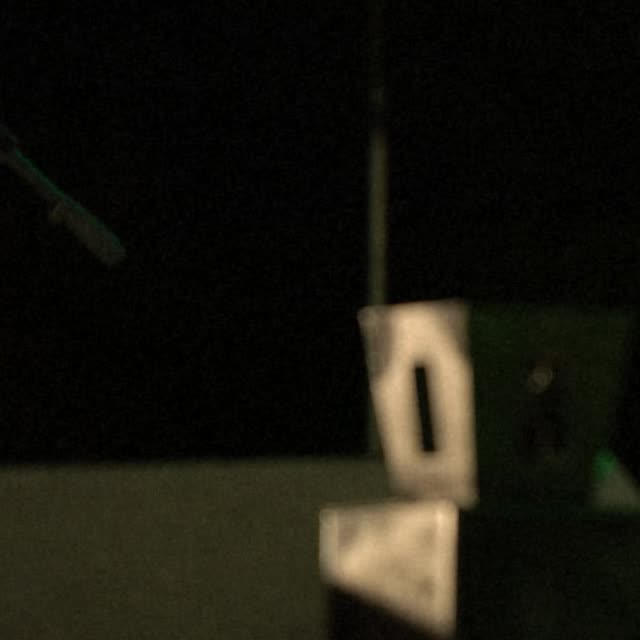
\includegraphics[width=0.47\columnwidth]{./img/noise_example.jpg}
\label{fig:sample}}
\subfigure[Noise features]{
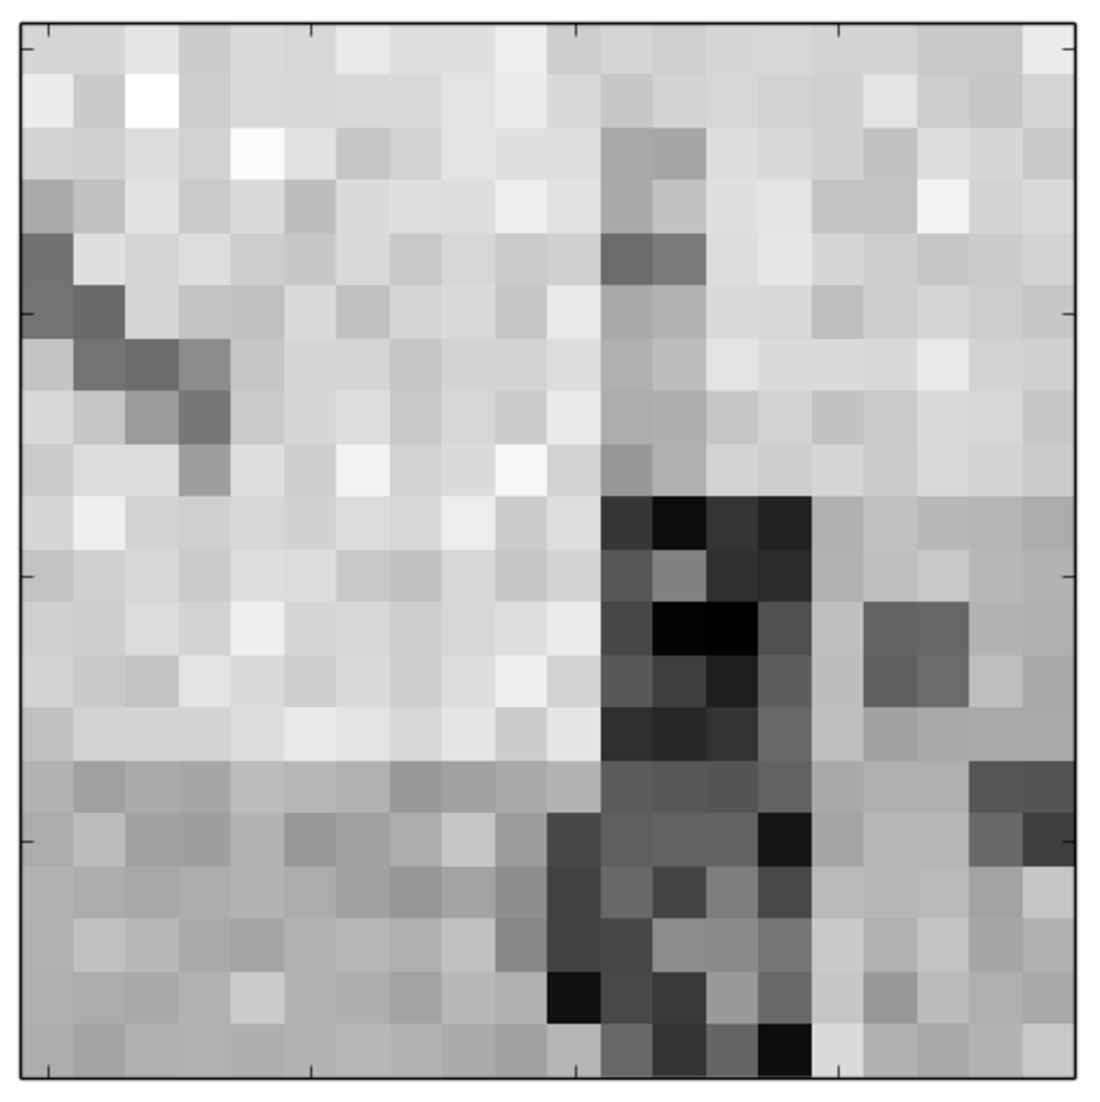
\includegraphics[width=0.47\columnwidth]{./img/r_feature_pub.eps}
\label{fig:r_feature}}
\subfigure[Visibility modulation factors]{
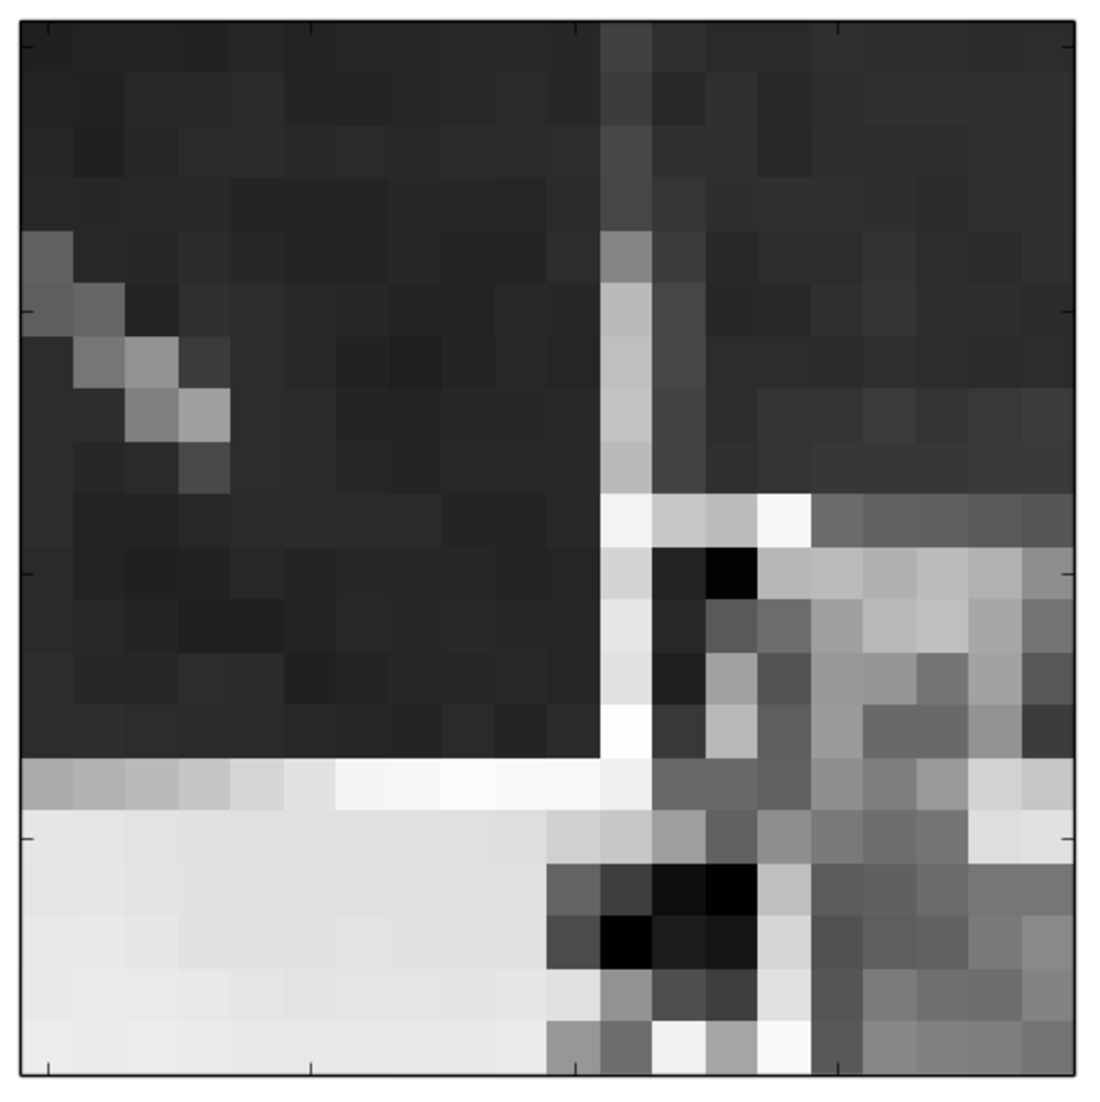
\includegraphics[width=0.47\columnwidth]{./img/w_feature_pub.eps}
\label{fig:w_feature}}
\subfigure[Visibility modulated noise features]{
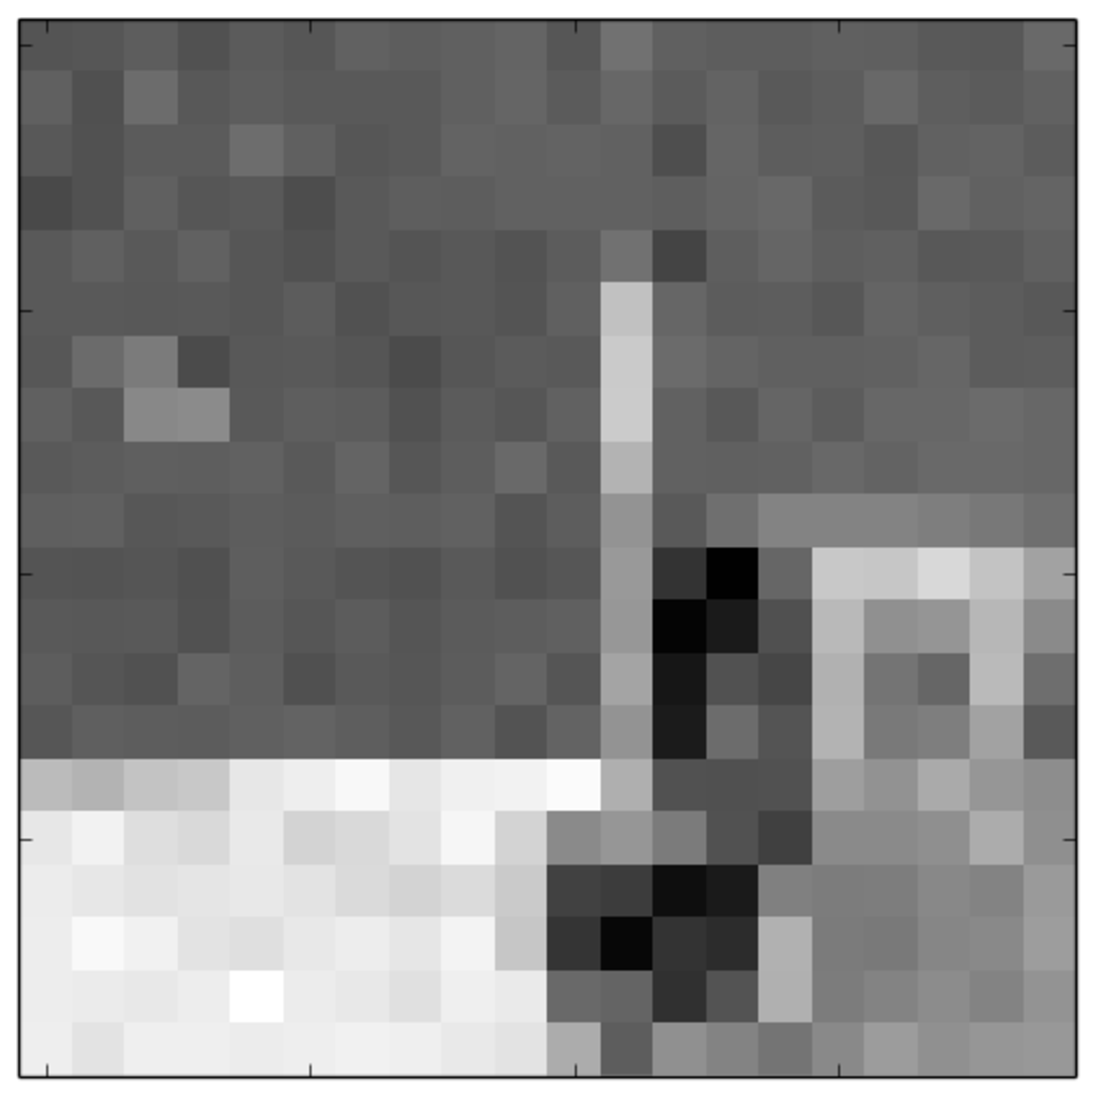
\includegraphics[width=0.47\columnwidth]{./img/m_feature_pub.eps}
\label{fig:m_feature}}
\caption{\label{fig:noise_visibility}\subref{fig:sample} A cropped sample frame from the test clip ``singer". \subref{fig:r_feature} The average noise feature $\frac{1}{B^2T}\sum_{\ell_x,\ell_y,\ell_t}\mathrm{r}(\ell_x,\ell_y,\ell_t)$ for all the $32\times32$ blocks;
\subref{fig:w_feature} The average visibility modulation factor $\frac{1}{B^2T}\sum_{\ell_x,\ell_y,\ell_t}\mathrm{w}(\ell_x,\ell_y,\ell_t)$ for all blocks;
\subref{fig:m_feature} The average modulated noise feature $\frac{1}{B^2T}\sum_{\ell_x,\ell_y,\ell_t}\mathrm{m}(\ell_x,\ell_y,\ell_t)$ for all blocks. Brighter color indicate larger value.
} 
\end{figure}

\begin{figure*}
\subfigure[$\ell_t=0$]{
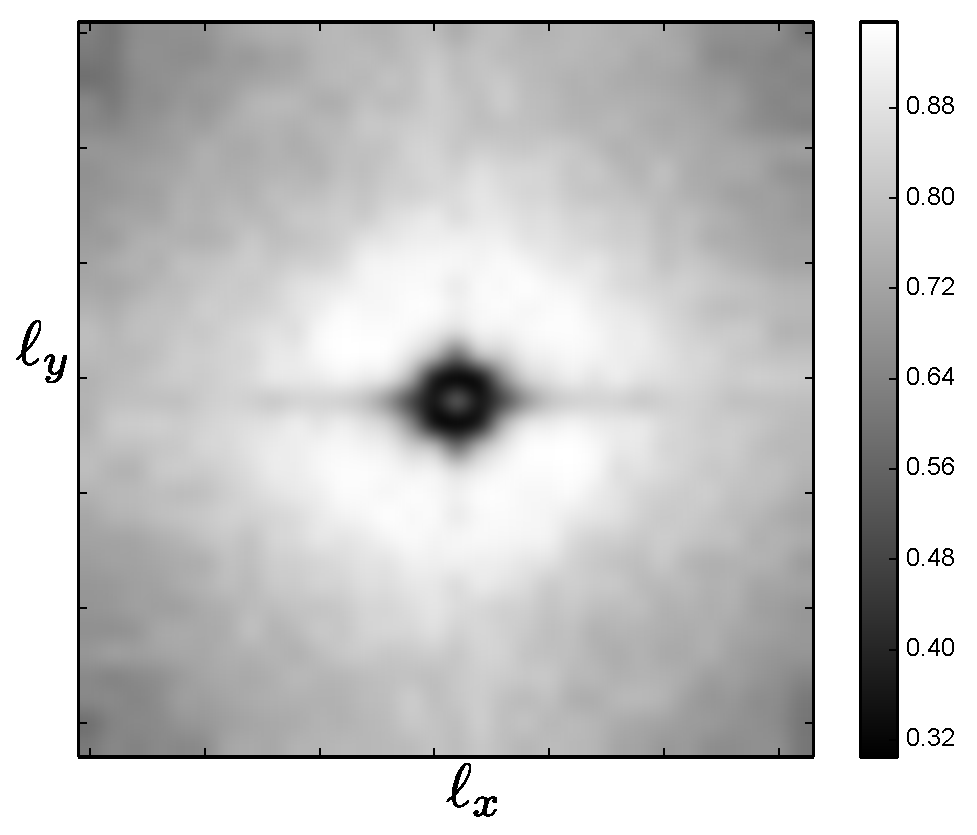
\includegraphics[width=0.33\textwidth]{./img/corr_0_pub.eps}
}
\subfigure[$\ell_t=1$]{
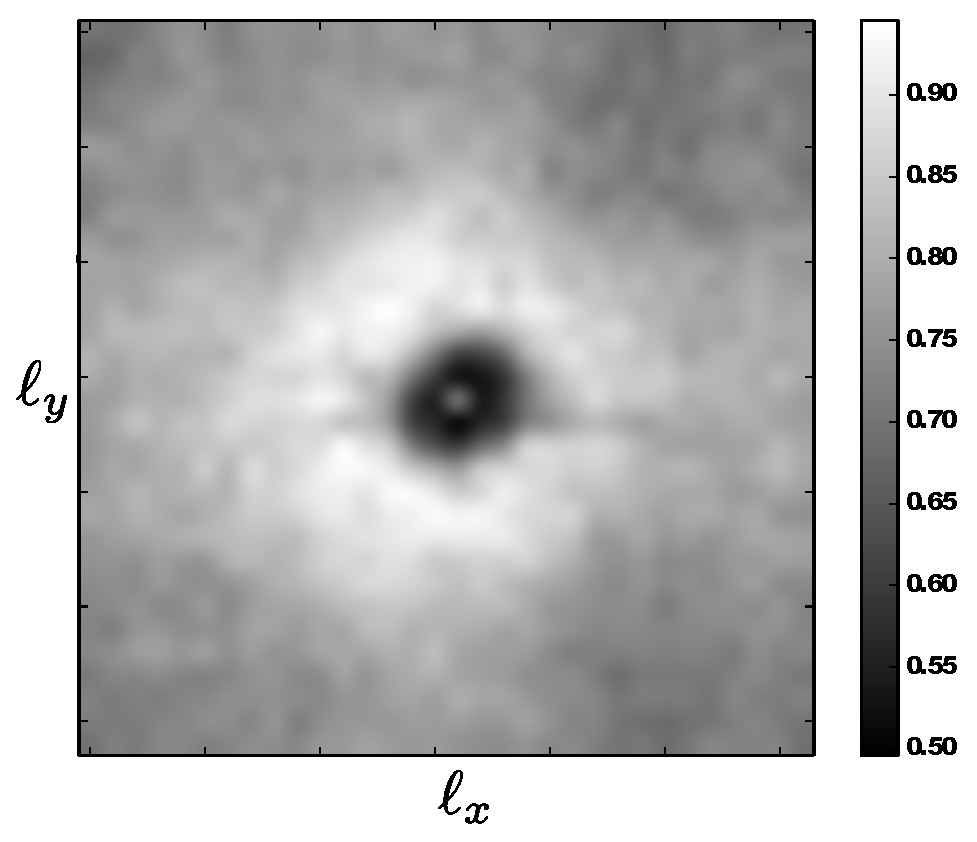
\includegraphics[width=0.33\textwidth]{./img/corr_1_pub.eps}
}
\subfigure[$\ell_t=2$]{
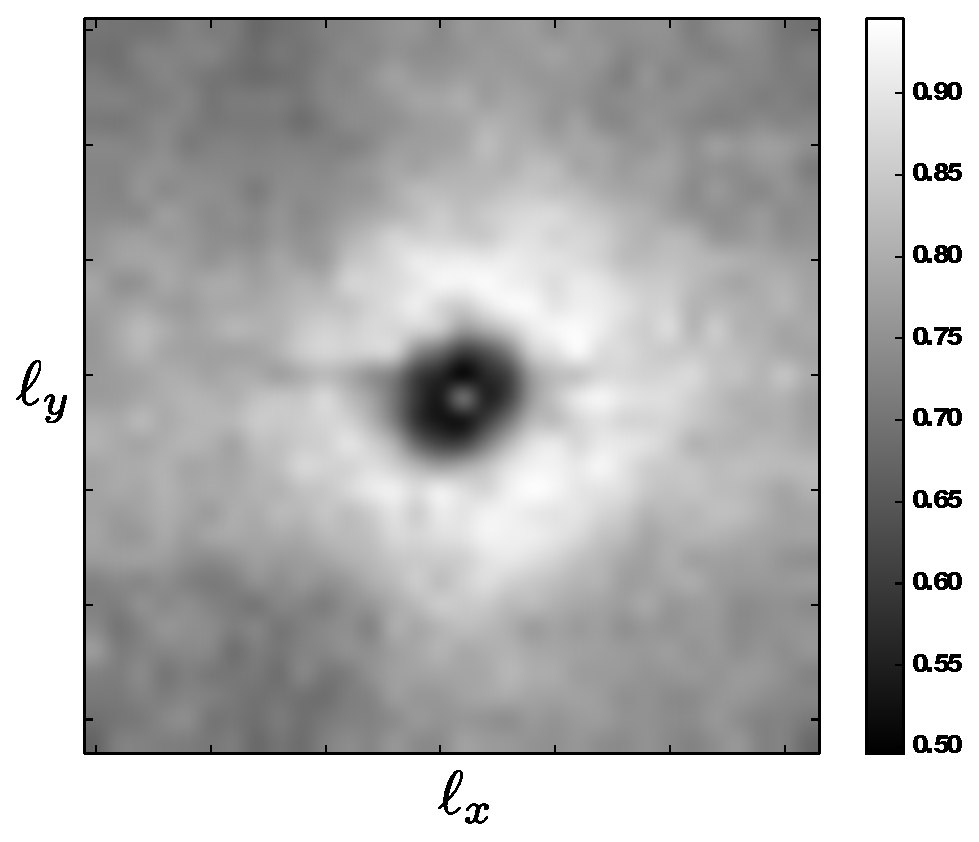
\includegraphics[width=0.33\textwidth]{./img/corr_2_pub.eps}
}
\caption{\label{fig:correlation_map}The absolute value of the rank-order correlation coefficient between $\mathrm{d}(\ell_x,\ell_y,\ell_t)$ with the MOS obtained from the subjective test. The coefficients are rearranged such that $\ell_x=0,\ell_y=0$ is located at the center of image.}
\end{figure*}
The visibility of noise depends on the background luminance. As shown in \cite{ChoLi1995,Gir1989}, in the dark regions of a video, the noise is much less visible than in the regions of mid-grey brightness. On the other hand, for regions of higher than mid-grey luminance, the noise visibility decreases with luminance, which is also known as Weber's law. To incorporate the impact of luminance, we modulate the distortion feature $\mathrm{r}^{p,q,t}(\cdot)$ by a function of local luminance. Assuming the luminance of pixels are normalized to $[0,1]$, we define the following function that approximately maps brightness to noise visibility: 
\begin{equation}
\label{eq:brightness}
\mathrm{w}(b) = \begin{cases}
b/\beta & 0\leq b\leq\beta,\\
1-(b-\beta)/(1-\beta) & \beta<b\leq1.
\end{cases}
\end{equation}
It is a piecewise linear function which connects points $(0,0)$, $(\beta,1)$, and $(1,0)$. The function $\mathrm{w}(b)$ is defined so as to capture the relationship between error visibility threshold and background luminance given by \cite{ChoLi1995}. The parameter $\beta$ is set to 0.15 to approximate the luminance under which the noise is most visible. Letting $b^{p,q,t}=\sum_{x,y}{\mathrm{v}(x,y,t)}/B^2$ be the average luminance of the $(p,q)$'th block, the visibility modulated noise feature of the block is given by
\begin{equation}
\label{eq:brightness_feature}
\mathrm{m}^{p,q,t}(\ell_x,\ell_y,\ell_t) = \mathrm{r}^{p,q,t}\left(\ell_x,\ell_y,\ell_t\right)\mathrm{w}\left(b^{p,q,t}\right).
\end{equation}

We show an example of the effect of this visibility modulation effect in Fig.~\ref{fig:noise_visibility}. Although equal amount of noise is added everywhere in the frame shown in Fig.~\ref{fig:noise_visibility}\subref{fig:sample}, the noise in the dark region is not quite visible. Fig.~\ref{fig:noise_visibility}\subref{fig:r_feature} shows that the perceptual noise level is overestimated by $\mathrm{r}(\ell_x,\ell_y,\ell_t)$ in the dark regions. By modulating the noise feature by $\mathrm{w}(\cdot)$ (see Fig.~\ref{fig:noise_visibility}\subref{fig:w_feature}), we can obtain a better estimation for the perceptual noise level (see Fig.~\ref{fig:noise_visibility}\subref{fig:m_feature}).


\subsection{Visual Importance Pooling}
In \cite{MooBov2009,ParSesLeeBov2013}, it has been recognized that the worst part of a video tends to attract more attention of the viewers and thus dominates the overall quality of the video. This fact has been exploited by a variety of visual importance pooling algorithms such as \cite{MooBov2009} and \cite{PinWol2004}. In our work, we applied a similar pooling method as \cite{MooBov2009}. For each frequency channel $(\ell_x,\ell_y,\ell_z)$, we first group the luminance modulated noise feature across all blocks, i.e., $\{\mathrm{m}^{p,q,t}(\ell_x,\ell_y,\ell_t): \forall p, \forall q\}$. Then we calculate the $p\%$ percentile of the features, denoted by $\mathrm{k}^{t}(\ell_x,\ell_y,\ell_t)$. Finally, we obtain the average distortion score for frequency $(\ell_x,\ell_y,\ell_z)$ as 
\begin{equation}
\mathrm{d}(\ell_x,\ell_y,\ell_t) = \frac{1}{\mathrm{F}}\sum_{t=1}^\mathrm{F}{\mathrm{k}^{t}(\ell_x,\ell_y,\ell_t)}. 
\end{equation}
where $\mathrm{F}$ is the number of frames of the video. In our implementation, the parameter $p$ for percentile pooling is set to 80\%.

\subsection{Frequency Selection}
The final step of our algorithm is to combine the distortion scores $\mathrm{d}(\cdot)$ for different spatial-temporal frequencies to predict MOS. For all the test clips in our subjective test, we calculated their distortion scores  $\mathrm{d}(\ell_x,\ell_y,\ell_t)$ for each frequency and then computed its rank-order correlation coefficients with the MOS obtained in our subjective test. The results are shown in Fig~\ref{fig:correlation_map}. It shows that for each temporal frequency $\ell_t$, the rank-order correlation coefficients are roughly concentric around the frequency $\ell_x=0,\ell_y=0$. In other words, the level of correlation mainly depends on the radial frequency $\ell_r=\sqrt{\ell_x^2 +\ell_y^2}$. At medium radial frequency, $\mathrm{d}(\ell_x,\ell_y,\ell_t)$ achieves very strong correlation with MOS (more than 0.9).

Based on the above observations, we use the sum of distortion scores on selected frequencies to predict the perceptual quality. The overall distortion metric is given by:
\begin{equation}
\label{eq:final_score}
\mathrm{D} = \sum_{t=0}^T\sum_{\ell_x=0}^{B}\sum_{\ell_y=0}^{B}\mathrm{d}(\ell_x,\ell_y,\ell_t)\mathrm{I}^{\ell_t}(\ell_x,\ell_y),
\end{equation} 
where $\mathrm{I}^{\ell_t}(\ell_x,\ell_y)$ is a binary frequency selection function. Because $\mathrm{d}(\ell_x,\ell_y,\ell_t)$ achieves maximum correlation with perceptual quality at medium radial frequencies, we use a simple ``band-pass" frequency selection function as follows:
\begin{equation}
\label{eq:freqency_selection}
\mathrm{I}^{\ell_t}(\ell_x,\ell_y) =
\begin{cases}
1 & \Psi_{\ell_t}\leq\sqrt{\ell_x^2 +\ell_y^2}\leq \Phi_{\ell_t},\\
0 & \text{otherwise},
\end{cases}
\end{equation}
where the parameters $\Psi_{\ell_t}$ and $\Phi_{\ell_t}$ defines the pass-band for the $\ell_t$'th temporal frequency plane. In our implementation, we choose $\Psi_0=\Psi_1=\Psi_2=4$, $\Phi_0=8$, and $\Phi_1=\Phi_2=6$.

\begin{figure*}
\subfigure{
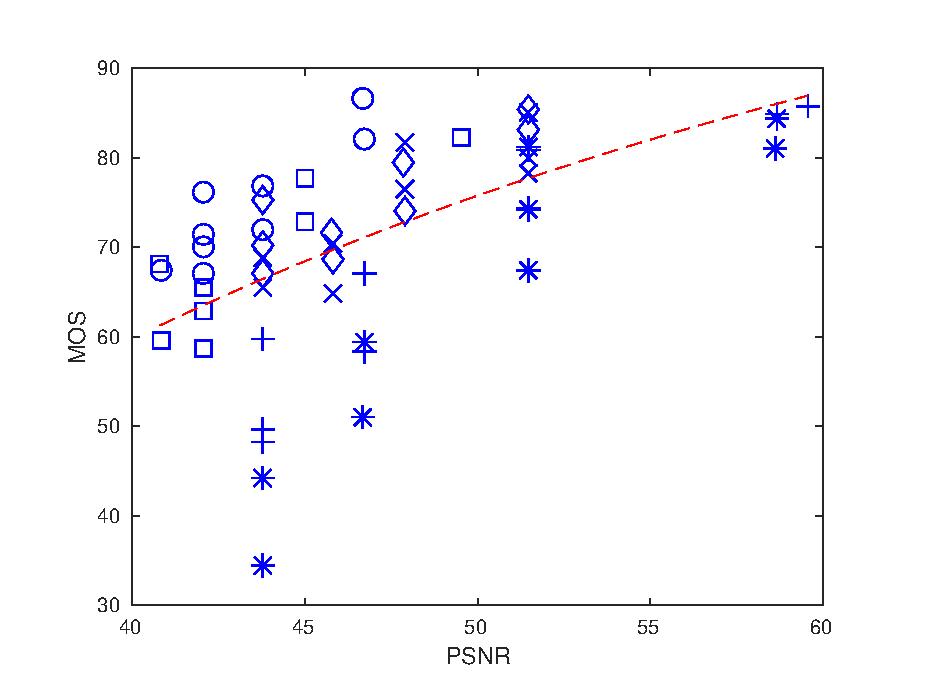
\includegraphics[width=\columnwidth]{./img/PSNR_fitting.eps}
}
\subfigure{
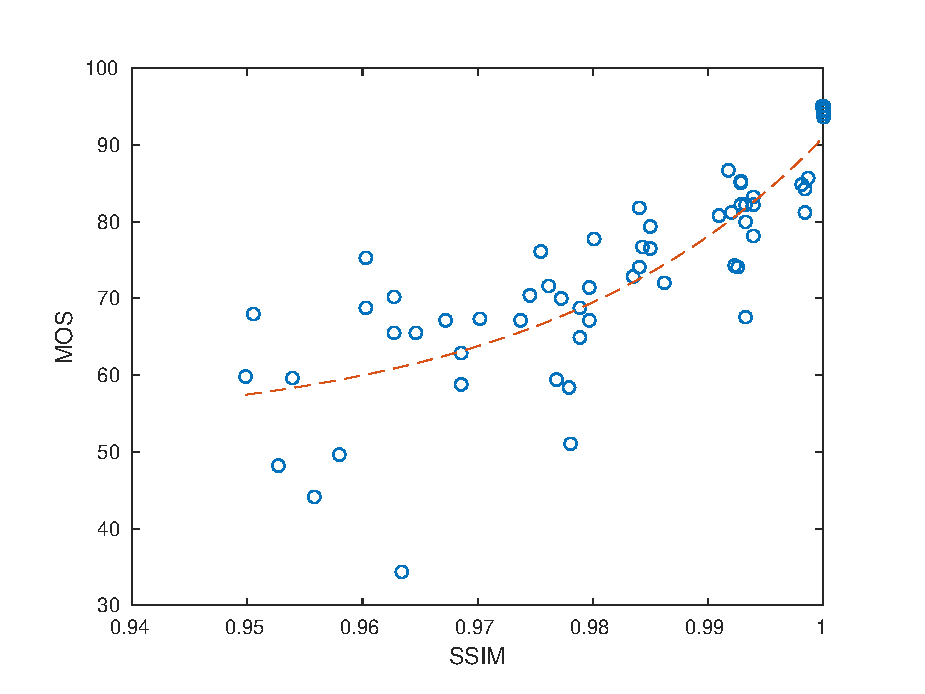
\includegraphics[width=\columnwidth]{./img/SSIM_fitting.eps}
}
\subfigure{
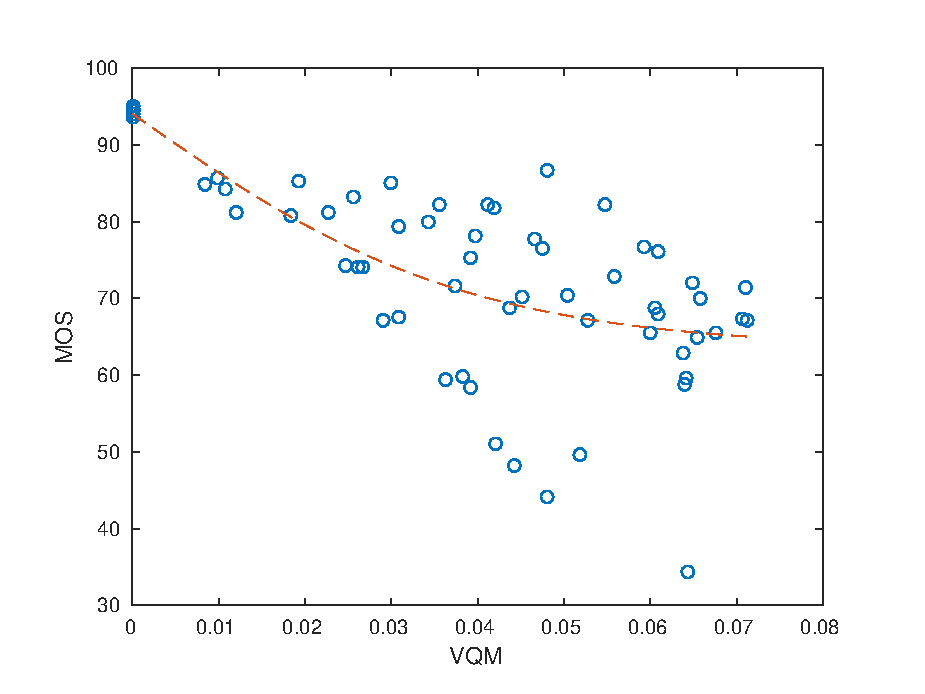
\includegraphics[width=\columnwidth]{./img/VQM_fitting.eps}
}
\subfigure{
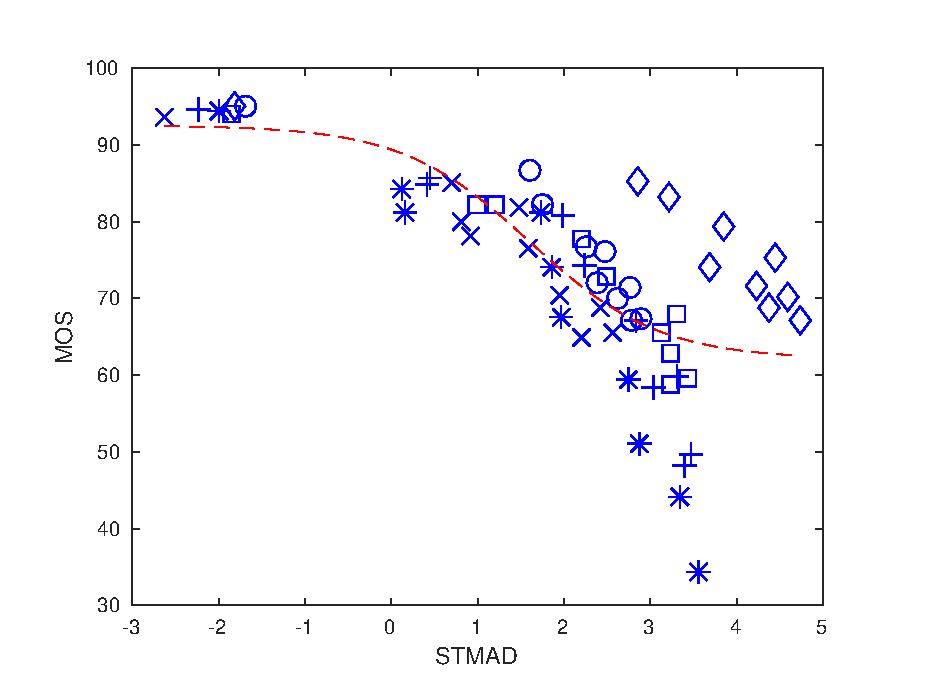
\includegraphics[width=\columnwidth]{./img/STMAD_fitting.eps}
}
\hspace*{1.7in}
\subfigure{
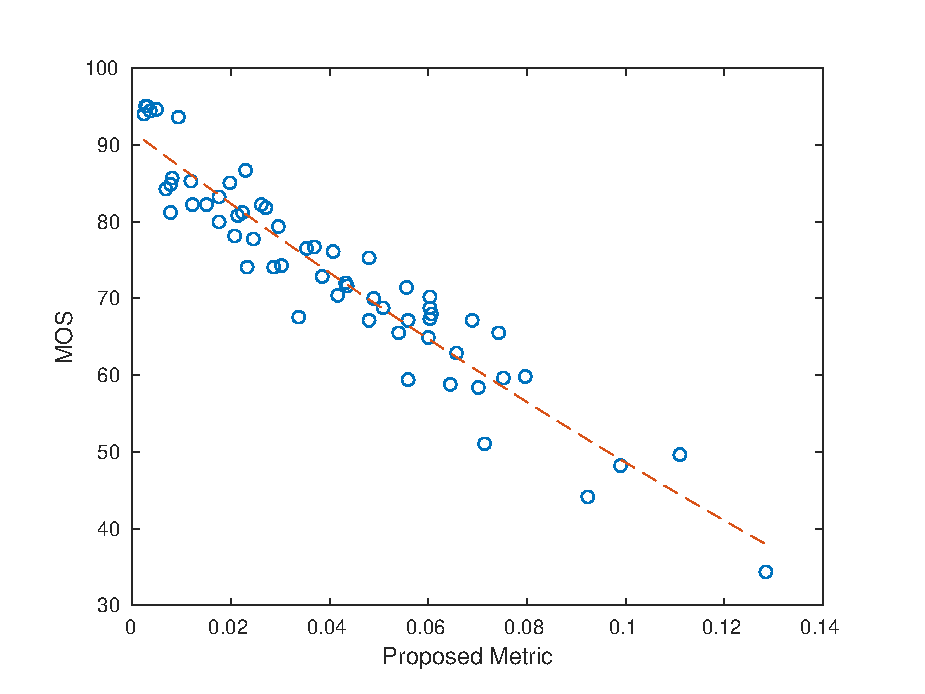
\includegraphics[width=\columnwidth]{./img/proposed_fitting.eps}
}
\caption{\label{fig:fitting} The regression results of PSNR, SSIM, VQM, STMAD, and the proposed noise metrics. The dashed lines show the fitted sigmoid model \eqref{eq:regression} for each metric.}
\end{figure*}


\section{Performance Evaluation}
\label{sec:experiment}
We evaluated the proposed metric on the videos tested in our subjective test. We employ the following polylog function to map our quality metric $D$ to the MOS. The fitted map is  
\begin{align*}
\label{eq:mos_mapping}
\mathrm{\hat{MOS}}(D) & = 2.5856\log^2(D) +23.3174\log(D) \\
&- 551.4506D + 143.6105.
\end{align*}
Our metric gives accurate predictions for perceptual quality. The linear correlation coefficient between the predicted MOS and the MOS is $0.9558$.

%\begin{figure}
%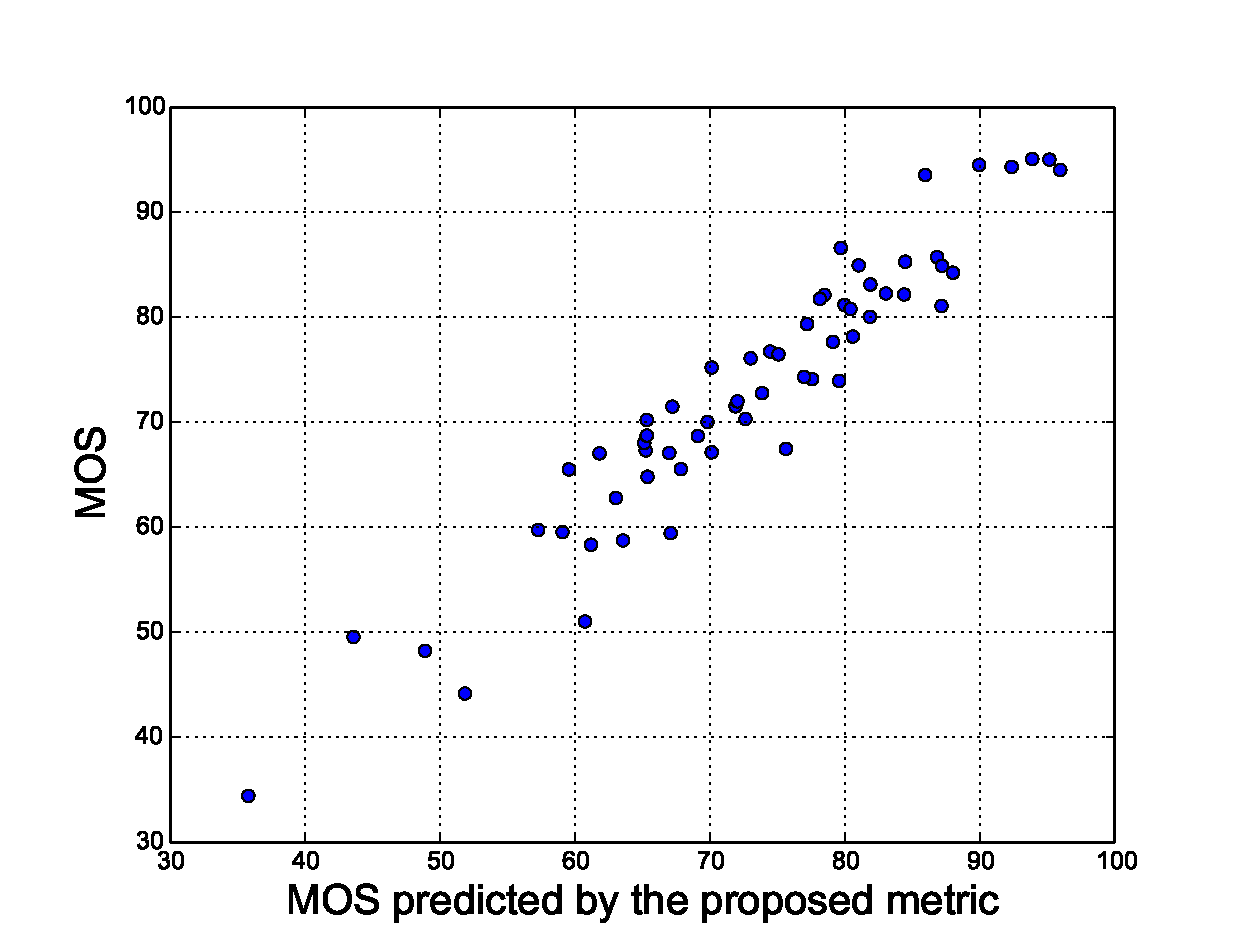
\includegraphics[width=\columnwidth]{img/preMos_Mos.eps}
%\caption{\label{fig:predicted_mos}The MOS predicted by the proposed metric versus the MOS %obtained from the subjective test.}
%\end{figure}

We also compared the performance of our metric with several widely used video quality metrics, including PSNR, SSIM, VQM, and STMAD. The comparison is based on three measurements: 1) rank order correlation coefficients (SROCC); 2) linear correlation coefficients (LCC) and variance of residuals (VoR) between predicted MOS and the empirical MOS. For each metric, we employ the following monotonic logistic regression model recommended by ITU in \cite{ITUValidation}:
\begin{equation}
\label{eq:regression}
\mathrm{MOS^{pred}} = \frac{a_1-a_0}{1+\left(\frac{M+a_4}{a_2}\right)^{a_3}} + a_0,
\end{equation}
where $M$ is the score given by a video quality metric and $\mathrm{MOS^{pred}}$ is the MOS predicted by the quality metric. The function parameters $a_0\cdots a_4$ are obtained by minimizing the mean square error of $\mathrm{MOS^{pred}}$. The results are shown in Fig.~\ref{fig:fitting}. The SROCC, LCC, and VoR of all the metrics are summarized in Table~\ref{tab:comparison}. The proposed algorithm outperforms all the other quality metrics in all the performance measurements. Note that PSNR, SSIM, VQM and STMAD all need to have access to the original noise-free video, which is typically unavailable for video sharing services such as YouTube. The proposed metric does not need the original video and is thus more appealing for consumer generated video contents.

\begin{table}
\centering
\caption{\label{tab:comparison}Performance comparison with other full-reference quality metrics.}
\resizebox{\columnwidth}{!}{
\begin{tabular}{|l|c|c|c|c|}
\hline
Quality Metrics&SROCC&LCC&VoR\\
\hline
Proposed&\bf{0.9518}&\bf{0.9497}&\bf{16.4933}\\
\hline
PSNR&0.6382&0.5838&86.4300\\
\hline
SSIM&0.8560&0.8287&52.7269\\
\hline
VQM&0.6707&0.6917&87.7917\\
\hline
STMAD&0.7412&0.7533&72.8135\\
\hline
\end{tabular}
}
\end{table} 

The parameters of our algorithm such as the numerical stabilizing constant $\alpha$ and visual importance pooling parameter $p$ are tuned using on our video database. To check if the database is large enough for training the algorithm parameters, we conducted cross-validations on our data base. Each time, we partition our database into a training set and a test set. We tune the parameters of our algorithm on the training set and evaluate the VoR on the test set. We vary the size of the training sets from 20\% to 90\% of the whole database. For a given training set size, cross-validations are repeated on 1000 random training/test set partitions and the average VoR is then calculated and shown in Fig.~\ref{fig:cross_validation}. It shows that the VoR decreases quickly as the size of training set increases. When the size of training set covers more than 60\% of the database, the average VoR does not decrease further. In other words, using 60\% of our database is enough for tuning the parameters of our model and the model parameter trained on our database is reliable. 
\begin{figure}
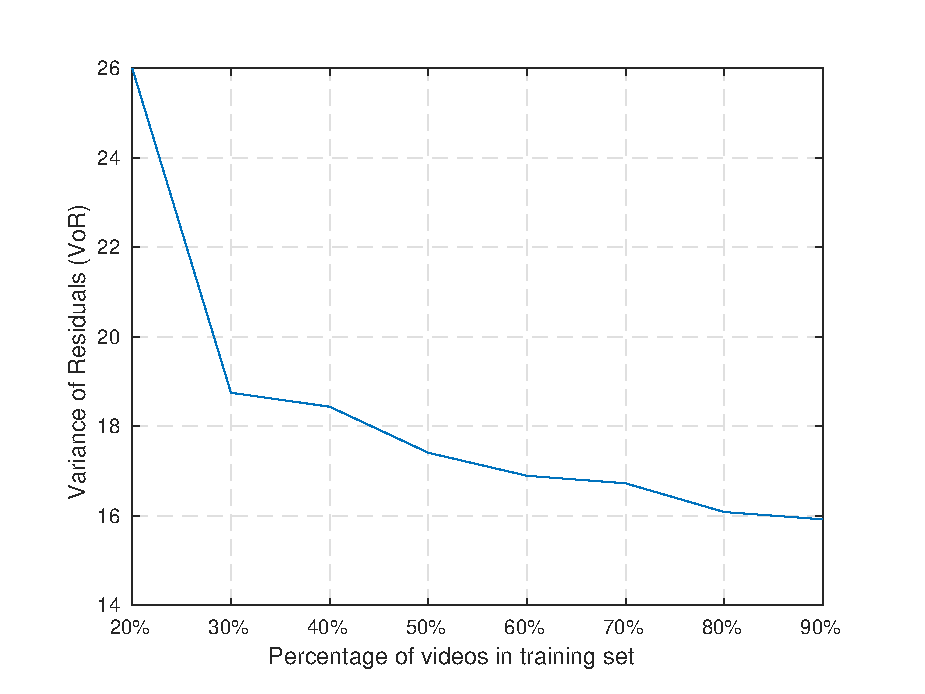
\includegraphics[width=\columnwidth]{./img/cross_validation.eps}
\caption{\label{fig:cross_validation} The variation of residuals (VoR) on the test set versus the size of the training set in cross validations.}
\end{figure}

\section{Conclusions and Future Work}
\label{sec:conclusion}
In this paper, we proposed a no-reference quality assessment algorithm for video distorted by noise. The algorithm captures the correlation structure of noise by using an estimated PSD. It also incorporated the impact of luminance and visual importance on the noise visibility in its design. The algorithm is trained and validated on a new database of noisy videos that simulates the typical noise patterns encountered in consumer-generated video content. The proposed algorithm can achieve up to 0.95 linear correlation with the MOS obtained from subjective studies, outperforming several high-performance video quality metrics.


%
% The following two commands are all you need in the
% initial runs of your .tex file to
% produce the bibliography for the citations in your paper.
\bibliographystyle{abbrv}
\bibliography{sigproc}  % sigproc.bib is the name of the Bibliography in this case
% You must have a proper ".bib" file
%  and remember to run:
% latex bibtex latex latex
% to resolve all references
%
% ACM needs 'a single self-contained file'!
%

\end{document}
